\documentclass{article}
\usepackage[english]{babel}
\usepackage[letterpaper,top=2cm,bottom=2cm,left=3cm,right=3cm,marginparwidth=1.75cm]{geometry}
\usepackage{amsmath}
\usepackage{graphicx}
\usepackage[colorlinks=true, allcolors=blue]{hyperref}
\usepackage[numbers]{natbib}
\usepackage{listings}

\title{Looking for Missing LowHadE Hits in Reconstructed Michels}
\author{Jozef Trokan-Tenorio}

\begin{document}
\maketitle

\section{Task Overview}

We have an excess of events with low visible hadronic energy (referred to as LowHadE events) in our data, shown in Fig. \ref{fig:cullen-hade-plot}. Specifically, this sample corresponds to events in the ND passing the full Numu2024ND selection, with an additinoal Cut on visible hadronic energy less than 0.01 GeV. 
\begin{figure}[htbp]
    \centering
    \IfFileExists{images-jtrokan/cullens-lowhade-plot.png}{%
        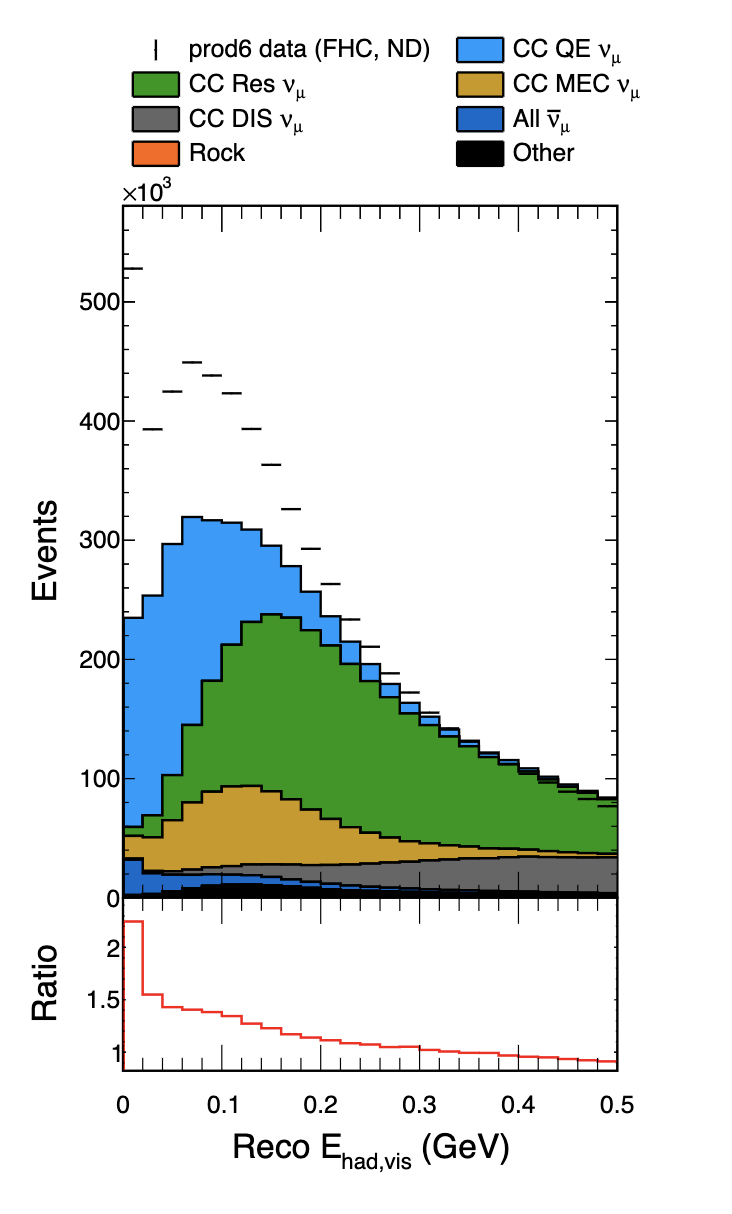
\includegraphics[width=0.5\textwidth]{images-jtrokan/cullens-lowhade-plot.png}%
    }{%
        \fbox{\parbox[c][0.25\textheight][c]{0.7\textwidth}{\centering Example image placeholder from \texttt{images-jtrokan/cullens-lowhade-plot}}}%
    }
    \caption{ Hadronic Visible Energy for fully inclusive ND numu CC selection in prod6. The large LowHadE data excess can be seen in the lowest energy bin here. Note that the LowHadE sample is defined by visible hadronic energy < 0.01 GeV, while the binning here is slightly larger (0.02 GeV bins) so the lowest bin in this plot contains the LowHadE sample and some other events. Taken from Cullen's technote \cite{2026-03-15-lowhade-excess}.  }
    \label{fig:cullen-hade-plot}
\end{figure}
Cullen has looked into the potential causes of this excess in extensive detail \cite{2026-03-15-lowhade-excess}. A small subset of the excess data events (5-15\%) have hits close to the vertex which appear to be the missing hadronic energy, but for some reason they were not sliced into the event with the track. An example is shown in Fig. \ref{fig:missing-hade-hits}. Some key information for this class of event is that these hits instead end up in the noise slice, and this class of event is only present in data, not MC (or at least, it is much more common in data than MC). 

\begin{figure}[htbp]
    \centering
    \IfFileExists{images-jtrokan/missing-hade-event.png}{%
        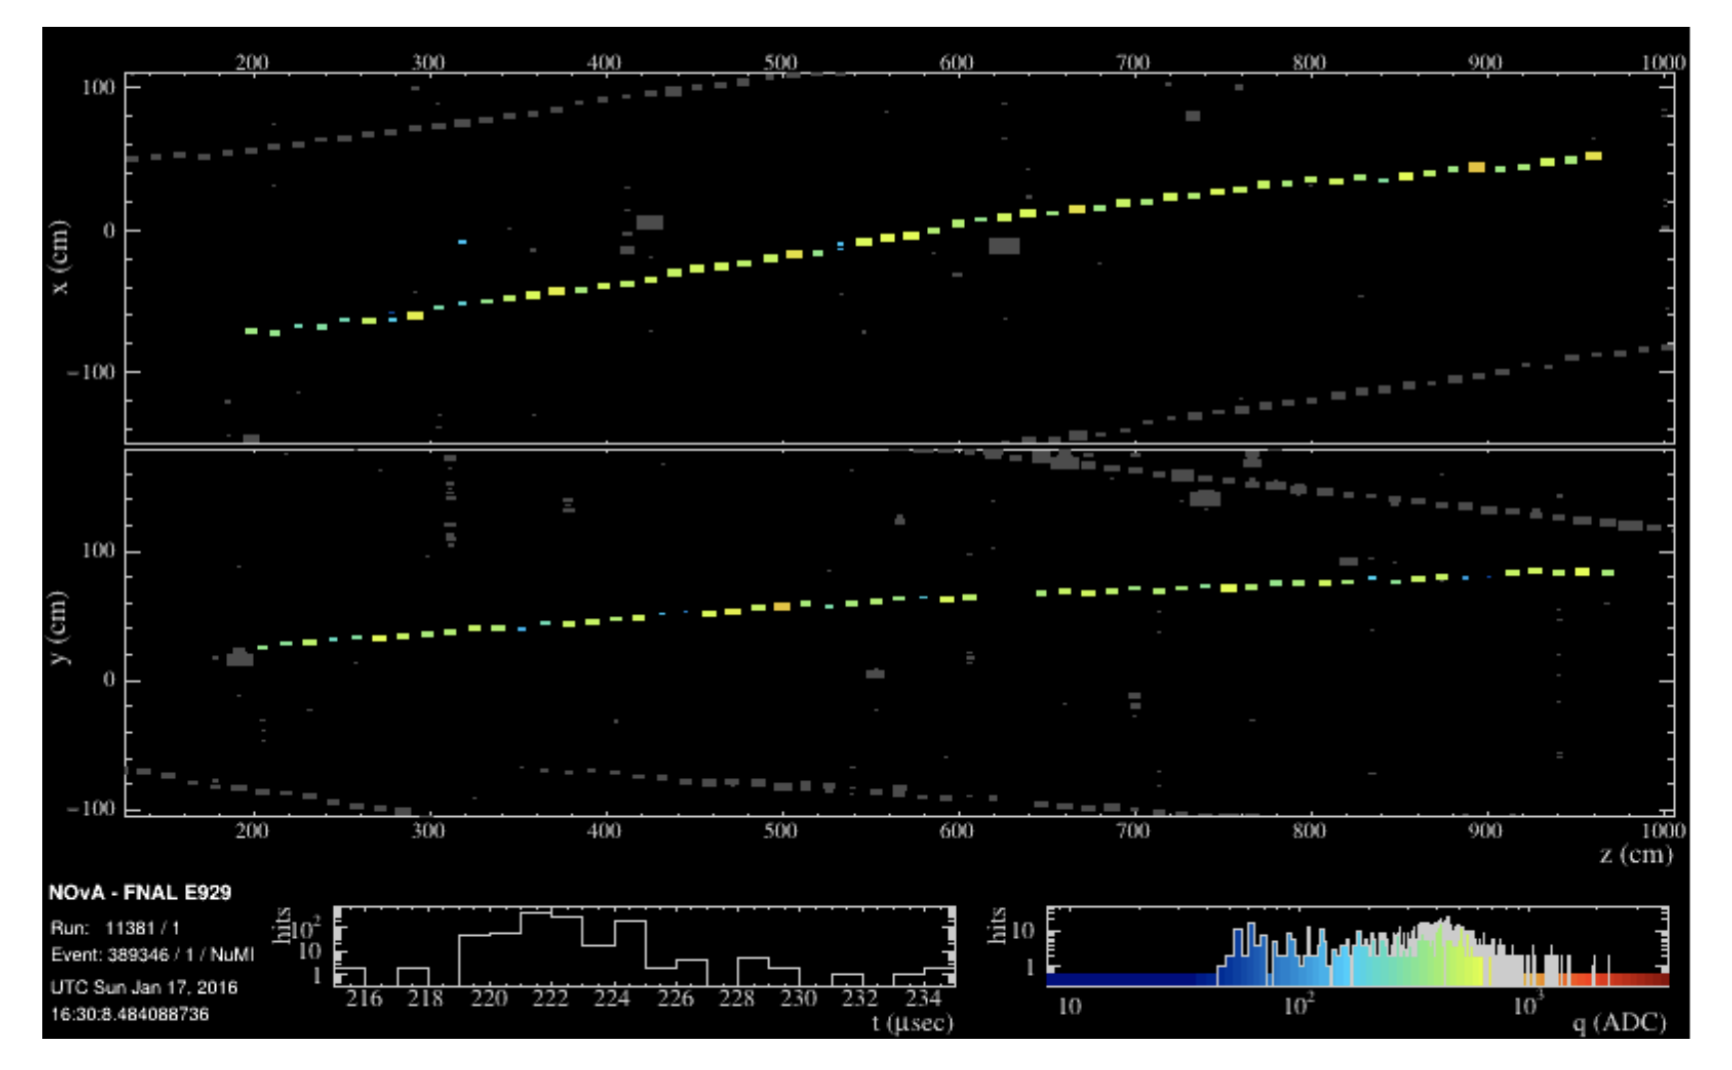
\includegraphics[width=0.7\textwidth]{images-jtrokan/missing-hade-event.png}%
    }{%
        \fbox{\parbox[c][0.25\textheight][c]{0.7\textwidth}{\centering Example image placeholder from \texttt{images-jtrokan/missing-hade-event.png}}}%
    }
    \caption{Hand-scanned LowHadE data event from Cullen’s technote with missing hits \cite{2026-03-15-lowhade-excess}. The missing hits can be seen as the greyed-out cluster near the start of the muon track on the left-hand side. }
    \label{fig:missing-hade-hits}
\end{figure}

We theorized that these missing hits could be getting mis-reconstructed as Michel electrons, and hoped that maybe this could be used as a path to reclaim that lost energy. Our reasoning was that the Michel electron reconstruction algorithm MEFinder looks for clusters of hits in the noise slice, which is exactly what these missing hits are. If the missing hits were indeed being reconstructed by MEFinder, they would show up as SlcME or TrkME located close to the start of the muon track. 

To check for this I took the LowHadE sample and plotted the distance between the muon track start and the reconstructed Michels, and if the missing hits were indeed being picked up by MEFinder I should see a large excess of Slc/TrkME in data, close to zero distance. We expect the data to have about 2.5x excess over MC just from the nominal LowHadE excess \cite{2026-05-11-lowhade-michels}, so if the missing hits were also being reconstructed the excess would be larger than this. 

Fig. \ref{fig:dist-to-trk-start} shows this plot, and it does have an excess, but it is not much more than the 2.5x nominal excess. To check this further I looked at the number of events. I plotted the energy distribution of Slc/TrkME that are close to the start of the muon track (within 50cm), to get these counts. That plot is shown in Fig. \ref{fig:vtxme-cale}. There are approximately 327,000 LowHadE events in data, and the ones with missing hits account for up to 15\%, or ~49,050 of those events. There are only \~6,500 reconstructed Slc/TrkME located close to the muon track start in data, with \~3,900 in MC. Even if all of the \~2,600 excess Slc/TrkME were from missing hadronic hits, it would only represent \~0.8\% of the LowHadE events. 

So, while there may be some missing hits getting mis-reconstructed as Michels, it is not nearly enough to account for this whole class of LowHadE events, and probably not a useful mechanism for reclaiming this lost energy. As for why we don't find more of the missing hits, I think it is most likely due to the selection cuts that MEFinder applies when making Michels. After identifying a cluster of hits, MEFinder will only make it a Slc/TrkME if it has less than 13 hits, and less than 100MeV of energy. These missing hits may simply have more than that so they are getting rejected by MEFinder. I have not actually gone and verified this it is just my conjecture at this point. 

\begin{figure}[htbp]
    \centering
    \IfFileExists{images-jtrokan/MichelDataMC_Numu2024ND_LowHadE_DistToTrkStart_prod6.png}{%
        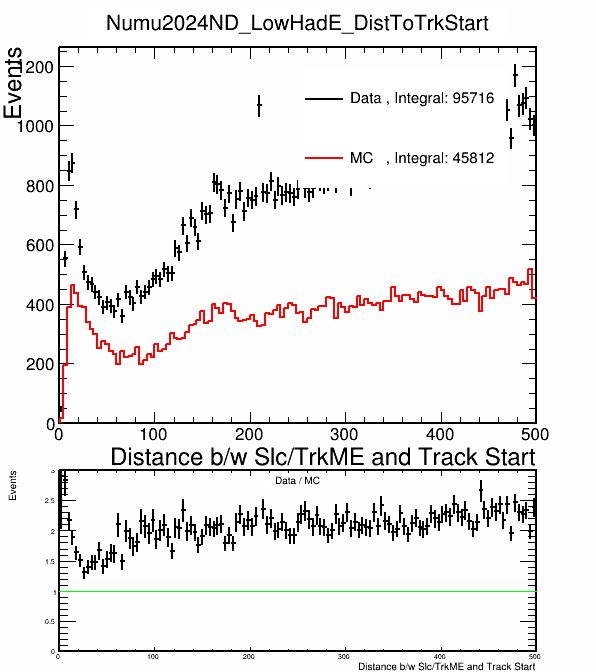
\includegraphics[width=0.7\textwidth]{images-jtrokan/MichelDataMC_Numu2024ND_LowHadE_DistToTrkStart_prod6.png}%
    }{%
        \fbox{\parbox[c][0.25\textheight][c]{0.7\textwidth}{\centering Example image placeholder from \texttt{images-jtrokan/missing-hade-event.png}}}%
    }
    \caption{ Distance between reconstructed Slc/TrkME and muon track start, for LowHadE events. X axis is shown in cm. The peak below 100cm corresponds to activity from and around the vertex. Around 100cm (or 1m) is around the minimum track length for muons in this sample (see my talk for the kalman track length plot \cite{2026-05-11-lowhade-michels}), so the points above that will start to include more actual Michel electrons at the ends of short tracks. For this study we really focus on the events below \~50cm. } 
    \label{fig:dist-to-trk-start}
\end{figure}

\begin{figure}[htbp]
    \centering
    \IfFileExists{images-jtrokan/MichelDataMC_Numu2024ND_LowHadE_VtxMECalE_prod6.png}{%
        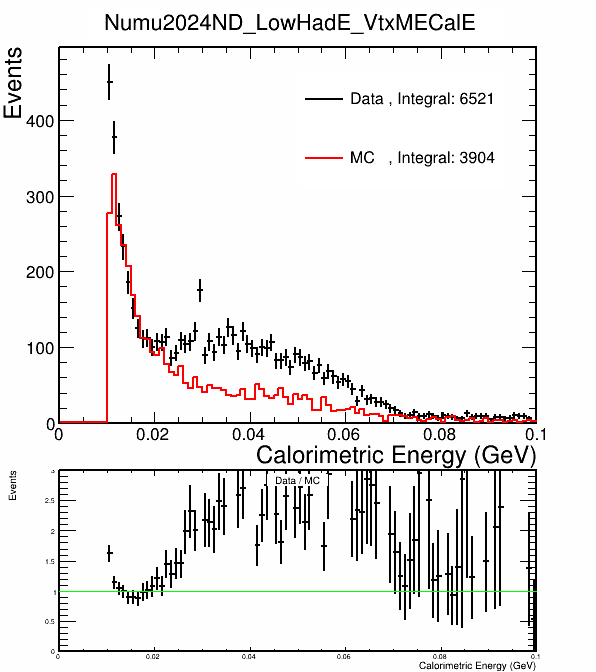
\includegraphics[width=0.7\textwidth]{images-jtrokan/MichelDataMC_Numu2024ND_LowHadE_VtxMECalE_prod6.png}%
    }{%
        \fbox{\parbox[c][0.25\textheight][c]{0.7\textwidth}{\centering Example image placeholder from \texttt{images-jtrokan/missing-hade-event.png}}}%
    }
    \caption{ Calorimetric energy of reconstructed SlcME and TrkME that are located close to the start of the muon track (within 50cm of the start) in LowHadE events. If you imagine a vertical line at 50cm in Fig. \ref{fig:dist-to-trk-start} this plot shows the energy of the events to the left of that line. }
    \label{fig:vtxme-cale}
\end{figure}


\section{Follow Ups}

Although we concluded that this is probably not where most of the missing hits are going, I received a few suggestions of things to follow up on (which I have not had time to do). One was to use this work to look for the corresponding missing hit events in MC. It's possible that these missing hit events are present in MC but just at a much lower rate. If I can identify them using the Michel reconstruction, we could then look at truth info to maybe understand them better, and maybe find out what is causing them to be missed. The idea would be to look at the Slc/TrkME in MC that are close to the muon track start, and identify a subset that correspond to the missing hits. These Slc/TrkME would not be true Michels, they would be a proton or pion or something. I could also check which of the reconstructed Slc/TrkME are matched to the correct parent slice. I think we would expect the missing hits to be Non-ME but still matched to the correct parent slice. Once I identify a possible sample in MC it would be good to check event displays to confirm the hits were indeed missed in the original event. This would be quite tricky as the event display is currently bugged and doesn't display MEFinder clusters (Slc/TrkME) correctly. So that would need to be fixed first. Another check that was suggested was to remake the distance to muon track start plot but normalize by number of numu events separately in data and MC (instead of normalizing both by POT), and that would remove the effect of the nominal LowHadE excess and only show any additional excess coming from the missing hits. 


\bibliographystyle{unsrtnat}
\bibliography{summary-jtrokan}

\end{document}
